\section{gitc extension}
\label{sec:Extension}
In this section we describe how a cloud9 user can work with our extension and we show how the developing workflow is improved by it.
Further we compare our extension to other tools introduced in section~\needcite{related work}.
Finally we will explain how we intregrated our extension to cloud9 and how we implemented it.

\subsection{Description}
\paragraph{The editor adjustments} of our extension will promt the cloud9 user immediately with visiual feedback of source code changes.
That means while typing within the editor annotations will appear next to the left grutter line as can be seen in figure~\ref{fig:editor}.

The changes show the staged and unstaged changes of the git repository respectively.
We choose to display those both types of changes as colored annotations whereas the already staged changes are more transparent.
In the upper screenshot of the cloud9 editor are only unstaged changes displayed.
The lower screenshot shows that the state of the git repository is changed.
Some of the changes are staged and at~\circnum{2} and~\circnum{3} are some (new) unstaged changes.
So in the line marked by~\circnum{2} there are both staged and unstaged changes visualized.
The colors green, blue and red are used to visualize added~\circnum{3}, changed~\circnum{2} and deleted~\circnum{1} lines respectively.

Furthermore the user will get tooltips hovering over one annotation.
In this way deleted lines or the old content of changed lines will be displayed to the user.
We do not provide buttons to stage, unstage or discard the changes because there is already an extension which allows developers to go back in history (see figure~\ref{fig:history}).
As for the staging and unstaging we want to have an overview over all current changes and thus rather use the diff view than search in single source code files for changes.

\begin{figure}
   \centering
   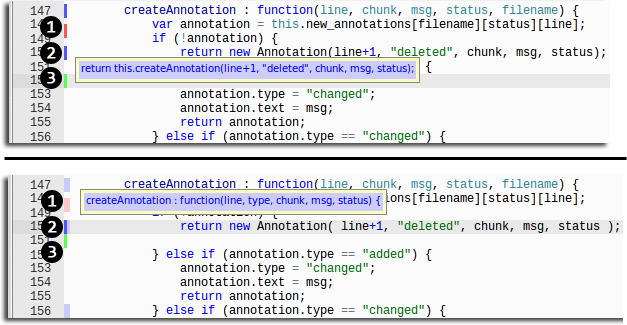
\includegraphics[width=0.9\textwidth]{images/extension_tooltip_comparison.png}
   \caption{Editor adjustments of our cloud9 extension gitc.}
   \label{fig:editor}
\end{figure}

\paragraph{Using our diff view} the cloud9 developer has now a view to explore \texttt{git diff} visually (see figure~\ref{fig:diff_view}).
By clicking on the pane button~\circnum{1} or simply using the keyboard shortcut \texttt{strg + g} / \texttt{cmd + g} the diff view will be opened.
The tree view at the left is filtered for changed files only.
The icon of an item of the tree will indicate the change state.
A green plus, a blue star and a red minus signify added, changed or deleted files respectively.
At the top~\circnum{2} the unstaged changes and at the bottom~\circnum{3} the staged changes are listed.

Double clicking on a file will open its changes in the editor.
Deleted or added lines will be marked with a red or green backgound and line numbers are displayed in two columns.
The left column shows the line number in the old file and the right column shows the line number in the new file.
For each single hunk there is a small menu with according options~\circnum{4}.
This is either to \emph{discard} or \emph{stage} unstaged hunks or \emph{unstage} staged hunks.
As soon as all belonging together hunks are staged developers can type summarizing message and click the commit button~\circnum{5}.
To pull and push from the git repository we provide context menu entries~\circnum{6}.

\begin{figure}
   \centering
   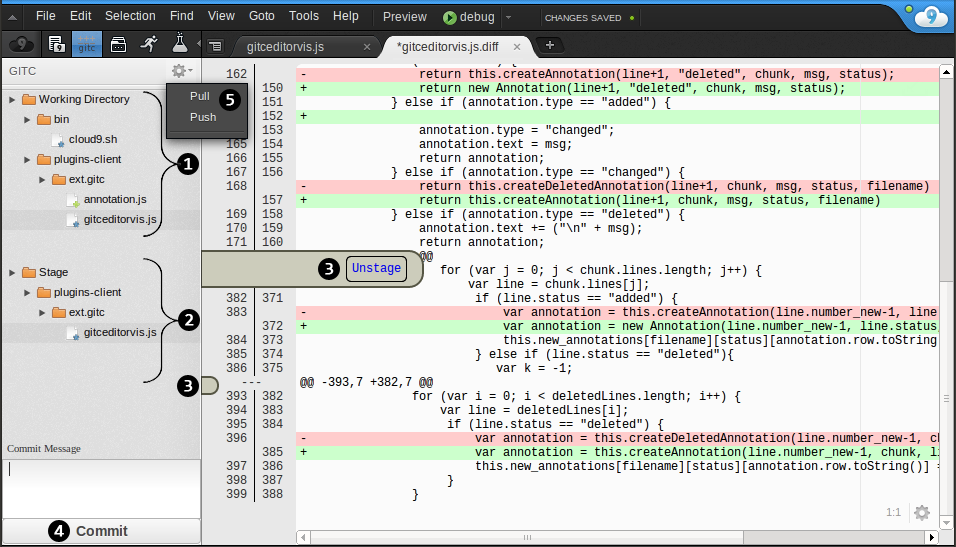
\includegraphics[width=0.9\textwidth]{images/extension_unstage.png}
   \caption{The diff view of our cloud9 extension gitc.}
   \label{fig:diff_view}
\end{figure}

\subsection{Workflow Improvement}
With our extension developers get realtime feedback of \texttt{git diff} of the current opened file while editing it.
This is visualized in a similiar way as stated in section~\ref{subsec:IntelliJ_IDEA}.
But we decided to not put buttons in our tooltip but to show the older content.
On the one hand because of the history extension (figure~\ref{fig:history}) enabling to discard changes.
On the other hand we figured out that mostly changes are scattered within one file or often over several files and thus buttons to stage and unstage hunks might not be that useful in a editor.
As a result there is no longer a need to switch back and forth from editor to console as we had before (see section~\needcite{our workflow}).

Once a developer decides to commit his changes he can switch via click or keyboard shortcut to our diff view.
Here it is possible to rapidly execute a bunch of git commands by simply clicking on certain buttons.
This replaces the missing interactive console to stage seperate code hunks and to only view a snippet of a diff.
Further we colorized changed lines as proposed in section~\ref{subsec:ext_git_integration} and~\ref{subsec:gitx}.

\todo[anything forgotten???]

\subsection{Implementation}
In the following subsections we will describe how we implemented our extension.
First we will have a closer look at how we intregrated our extension to cloud9 and how we execute git commands.
Then we will explain how we implemented the adjustments in the cloud9 editor and the new diff view.

\subsubsection{Integration to cloud9}
%Stephi
client-side, server-side hook
sending commands (channel)
reacting to commands
git parser
following two are as well client-side

\subsubsection{Editor Adjustments}
%Patrick

\subsubsection{Diff View}
%Markus
